\documentclass{article}
\usepackage[margin=0.3in]{geometry}
\usepackage{amsmath}
\usepackage{amsfonts}
\usepackage{amssymb}
\usepackage{amsthm}
\usepackage{parskip}
\usepackage{multicol}
\usepackage{xcolor}
\usepackage{fancyhdr}
\usepackage{physics}
\usepackage{graphicx} % Required for inserting images
\usepackage{hyperref}
\usepackage{enumitem}
\newcommand{\matr}[1]{\mathbf{#1}}
\def\dbar{{\mathchar'26\mkern-12mu d}}

\newtheorem{definition}{Definition}[section]
\newtheorem{theorem}{Theorem}[section]
\newtheorem{corollary}{Corollary}[theorem]
\newtheorem{lemma}[theorem]{Lemma}

\pagestyle{fancy}
\fancyhf{}
\renewcommand{\headrulewidth}{1pt}
\fancyhead[R]{\thepage}

\begin{document}

\begin{multicols}{3}
\noindent

\subsubsection*{Integrating factors}
$$y'+P(x)y=Q(x)$$
$$I(x)=\exp\left(\int P(x)dx\right)$$
$$y(x)=\frac{1}{I(x)} \int Q(x)I(x)dx + \frac{\alpha}{I(x)}$$

\subsubsection*{Change of variables}
$$y^{(n)} = F(y, y', \dots, y^{(n-1)}, t)$$
Let $x_{i+1} = y^{(i)}$ where $i \in \{0, 1, \dots, n-1\}$.

\subsubsection*{Picard-Lindel{\"o}f statement}
Consider IVP: $x_{i}'=F_i(t, x_1, \dots, x_n)$ \\
or that $\boldsymbol{x}'=\boldsymbol{F}(t,\boldsymbol{x})$
with $\boldsymbol{x}(t_0)=\boldsymbol{x}_0$ \\
and $\boldsymbol{x}$ is a vector with $n$ entries.

It has \textbf{unique} solutions if:
$$F_i, \frac{\partial F_i}{\partial x_j}
\hspace{0.05in}\text{and}\hspace{0.05in}
\frac{\partial F_i}{\partial t}
\hspace{0.05in}\text{are \underline{continuous} in}$$
$R\subset\mathbb{R}^{n+1}$ where $(t,\boldsymbol{x}_0^{T})\in R$. \\
Here $i, j \in \{1, \dots, n\}$.

\subsubsection*{Homogeneous systems}
Consider $\boldsymbol{x}'=\matr{A}\boldsymbol{x}$
where $\matr{A}$ is a $n \times n$ matrix.
Substituting $\boldsymbol{x}=e^{rt} \boldsymbol{\xi}$ gives:
$$(\matr{A}-r_i \matr{I_n})
\boldsymbol{\xi^{(i)}}=\boldsymbol{0}$$
where $i\in\{1,2,\dots, n\}$. \\ Our general solution is then:
\begin{align*}
    \boldsymbol{x}(t)
    &=\sum_{i=1}^{n}c_i e^{r_i t}\boldsymbol{\xi}^{(i)} \\
    &=\sum_{i=1}^{n}c_i\boldsymbol{x}^{(i)} \\
    &=\boldsymbol{\Psi}(t)\boldsymbol{c}.
\end{align*}
If initial conditions $\boldsymbol{x}(t_0)=\boldsymbol{x}_0$
are given:
$$\boldsymbol{c}=\boldsymbol{\Psi}^{-1}(t_0)\boldsymbol{x}(t_0)$$
$$\boldsymbol{x}(t)=\boldsymbol{\Psi}(t)
\boldsymbol{\Psi}^{-1}(t_0)\boldsymbol{x}_0.$$

\subsubsection*{Matrix exponentials}
Given a $n\times n$ matrix $\boldsymbol{A}$:
\begin{align*}
    e^{\boldsymbol{A}t}
    &=\sum_{n=0}^{\infty}
    \frac{(\boldsymbol{A}t)^n}{n!} \\
    &=\boldsymbol{I}_n
    +\boldsymbol{A}t
    +\frac{1}{2!}\boldsymbol{A}^2t^2+\dots.
\end{align*}
For system 
$\boldsymbol{x}'=\boldsymbol{A}\boldsymbol{x}$:
$$\boldsymbol{x}(t)
=e^{\boldsymbol{A}t}\boldsymbol{x}(0)$$
and that $e^{\boldsymbol{A}t}
=\boldsymbol{\Psi}(t)\boldsymbol{\Psi}^{-1}(0)$.

\subsubsection*{Diagonalisation}
For $\boldsymbol{x}'
=\boldsymbol{A}\boldsymbol{x}$ we have
$\boldsymbol{A}=\boldsymbol{T}
\boldsymbol{D}\boldsymbol{T}^{-1}$. \\
If $\boldsymbol{x}=\boldsymbol{T}
\boldsymbol{y}$ then $\boldsymbol{y}'=\boldsymbol{D}\boldsymbol{y}$.

Since our fundamental matrix with respect to
$\boldsymbol{y}$ is a \underline{diagonal} matrix
$\boldsymbol{Q}=e^{\boldsymbol{D}t}$,
the fundamental matrix with respect to
$\boldsymbol{x}$ is
$\boldsymbol{\Psi}(t)
=\boldsymbol{T}e^{\boldsymbol{D}t}$
and:
$$e^{\boldsymbol{A}t}=\boldsymbol{T}
e^{\boldsymbol{D}t}\boldsymbol{T}^{-1}.$$

\subsubsection*{Generalised eigenvectors}
If eigenvalues do not generate enough eigenvectors to
form $n$ linearly independent solutions for a
$n\times n$ matrix $\boldsymbol{A}$, 
then consider the following ansatz:
$$\boldsymbol{x}=te^{rt} \boldsymbol{\xi}+e^{rt} \boldsymbol{\eta}.$$
$$\therefore(\matr{A}-r_i \matr{I_n})\boldsymbol{\eta^{(i)}}=\boldsymbol{\xi^{(i)}}$$
Then this $r_i$ produces \underline{two} solutions:
$$\boldsymbol{x}^{(1)}=e^{rt}\boldsymbol{\xi}$$
$$\boldsymbol{x}^{(2)}
=te^{rt} \boldsymbol{\xi}+e^{rt} \boldsymbol{\eta}.$$
    
\subsubsection*{Non-homogeneous systems}

Consider non-homogeneous ODE system:
$$\boldsymbol{x}'=\boldsymbol{A}\boldsymbol{x}+\boldsymbol{g}.$$
\begin{itemize}
    \item \textbf{Change of basis}
        
    Let $\boldsymbol{x}=\boldsymbol{T}\boldsymbol{y}$
    and since $\boldsymbol{A}=\boldsymbol{T}\boldsymbol{D}\boldsymbol{T}^{-1}$:
    $$\boldsymbol{y}'=\boldsymbol{D}\boldsymbol{y}+\boldsymbol{T}^{-1}\boldsymbol{g}$$
    which is solved by integrating factors. Finally \underline{revert back} to $\boldsymbol{x}$.

    \item \textbf{Variation of parameters}

    Find solution $\boldsymbol{x}_H=\boldsymbol{\Psi}\boldsymbol{c}$ 
    to $\boldsymbol{x}'=\boldsymbol{A}\boldsymbol{x}$.
    Then let the non-homogeneous solution be
    $\boldsymbol{x}=\boldsymbol{\Psi}\boldsymbol{u}(t)$.
    $$\therefore\boldsymbol{\Psi}\boldsymbol{u}'(t)=\boldsymbol{g}(t)$$
    Row reduce before integrating.

    \item \textbf{Undetermined coefficients}

    Let non-homogeneous ODE system have solutions of form:
    $$\boldsymbol{x}=\boldsymbol{x}_H + \boldsymbol{x}_p$$
    where $\boldsymbol{x}_H$ is our homogeneous solution
    and $\boldsymbol{x}_p$ our \underline{particular} solution.        
    \end{itemize}

\subsubsection*{Critical points}
Consider non-linear ODE system
$$x'=F(x, y),$$
$$y'=G(x, y).$$
We define $\boldsymbol{x^0}=\begin{bmatrix} x^0 \\ y^0 \end{bmatrix}$
as a \textbf{critical point} when $F(\boldsymbol{x^0})=G(\boldsymbol{x^0})=0$.

\subsubsection*{Linearisation and stability}
Let $\boldsymbol{u}=\begin{bmatrix} u_1 \\ u_2 \end{bmatrix}
=\begin{bmatrix} x-x^0 \\ y-y^0 \end{bmatrix}$.
\begin{align*}
    \therefore u_1'
    &\approx F(x^0, y^0)+\left(\frac{\partial F}{\partial x}\right)_{x^0}(x-x^0) \\
    &+\left(\frac{\partial F}{\partial y}\right)_{y^0}(y-y^0) \\
    \therefore u_2 
    &\approx G(x^0, y^0)+\left(\frac{\partial G}{\partial x}\right)_{x^0}(x-x^0) \\
    &+\left(\frac{\partial G}{\partial y}\right)_{y^0}(y-y^0) \\
    \therefore\boldsymbol{u}' &= \boldsymbol{A}\boldsymbol{u} \\
    &=\begin{bmatrix}
        \partial F/\partial x & \partial F/\partial y \\
        \partial G/\partial x & \partial G/\partial y
    \end{bmatrix}_{\boldsymbol{x} = \boldsymbol{x^0}}
    \textcolor{red}{\begin{bmatrix} x-x^0 \\ y-y^0 \end{bmatrix}}
\end{align*}
Critical points $\boldsymbol{x^0}$ may also be classified: \\
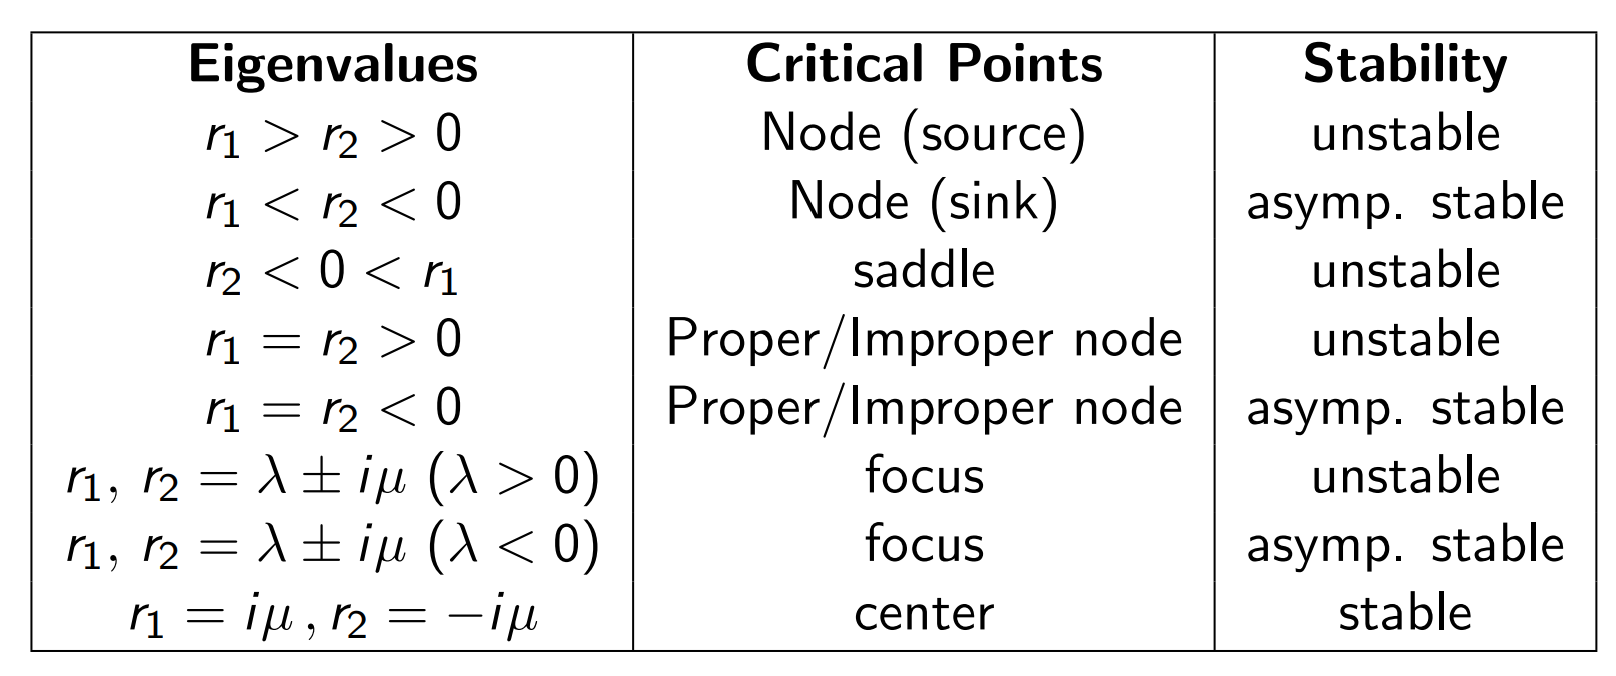
\includegraphics[scale=0.33]{f1.png}
Linearisation preserves critical point behaviour \textbf{except} when eigenvalues are of $r=\pm i\mu$ form,
for which then classification is unknown.

\textbf{Stable} critical points $\boldsymbol{x^0}$: \\
All solutions \underline{start} and \underline{stay near} $\boldsymbol{x^0}$.
\begin{align*}
    &\forall\epsilon>0;\exists\delta>0;\forall
    \boldsymbol{x}(t)=\boldsymbol{\phi}(t):
    |\boldsymbol{x}(0)-\boldsymbol{x^0}|<\delta \\
    &\implies |\boldsymbol{x}(t)-\boldsymbol{x^0}|<\epsilon
    \hspace{0.05in}\text{for}\hspace{0.05in}\forall t \geq 0
\end{align*}

\textbf{Attracting} critical points $\boldsymbol{x^0}$: \\
All solutions \underline{tends} to $\boldsymbol{x^0}$.
\begin{align*}
    &\forall\delta>0:|\boldsymbol{x}(0)-\boldsymbol{x^0}|<\delta \\
    &\implies\lim_{t\rightarrow\infty}
    \boldsymbol{x}(t)=\boldsymbol{x^0}
\end{align*}

\textbf{Asymptotically stable} critical points $\boldsymbol{x^0}$:
Attracting \textbf{and} stable.

\subsubsection*{Lyapunov's theory and limit cycles}
Consider $\dot{x}=F(x, y)$ and $\dot{y}=G(x, y)$
and let $\boldsymbol{x^0} \in D$ be a critical point.
Let $E:D\subset\mathbb{R}^2\rightarrow\mathbb{R}$
is defined such that $E(x^0, y^0)=0$.
$$\therefore\frac{\dd E}{\dd t}=\frac{\partial E}{\partial x} F
+\frac{\partial E}{\partial y} G$$
\begin{itemize}
    \item Let $E>0$ for $\forall \boldsymbol{x} \neq \boldsymbol{x^0}$.
        
    If $\frac{\dd E}{\dd t} \leq 0$ then $\boldsymbol{x^0}$ is stable.

    If $\frac{\dd E}{\dd t} < 0$ then $\boldsymbol{x^0}$ is asymptotically stable.

    \item $E(\boldsymbol{x^*})>0$ and $\frac{\dd E}{\dd t}>0$
    
    $\implies$ unstable $\boldsymbol{x^0}$.
    (flip both signs)
\end{itemize}

\newpage

Postive definite:
$E(\boldsymbol{x})>0$ for
$\forall\boldsymbol{x}\neq\boldsymbol{x^0}$

Postive semidefinite: \\
$E(\boldsymbol{x})\geq0$ for
$\forall\boldsymbol{x}\neq\boldsymbol{x^0}$

\textbf{Limit cycles} are periodic solutions such that 
at least one other \textcolor{red}{non-closed trajectory}
approaches it as $t\rightarrow\infty$.

Generally if our trajectory is \underline{enclosed}
by finite non-simple region and $F$, $G$ have 
continuous partials then there is a limit cycle.

\subsubsection*{Real Fourier series}
The Fourier expansion of piecewise continuous
$f(x)$ on $[-L,L]$ is:
$$f_{FS}(x)=\frac{a_0}{2}+\sum_{n=1}^{\infty}
(a_n \cos\frac{n\pi x}{L}+b_n \sin\frac{n\pi x}{L})$$
where $f_{FS}(x)=f_{FS}(x+\boldsymbol{2L})$.
If $\alpha$ is a discontinuous point:
$$f_{FS}(\alpha)=\frac{f(\alpha^{+})+f(\alpha^{-})}{2}$$
for $\alpha^{+}$ is the limit from the \underline{left}.

Our Fourier coefficients are:
$$a_0=\frac{1}{L}\int_{-L}^{L}f(x)\dd x$$
$$a_n=\frac{1}{L}\int_{-L}^{L}\cos\frac{n\pi x}{L}f(x)\dd x$$
$$b_n=\frac{1}{L}\int_{-L}^{L}\sin\frac{n\pi x}{L}f(x)\dd x.$$

\subsubsection*{Orthogonality}
Let $S_n = \sin\frac{n\pi x}{L}$ and $C_n = \cos\frac{n\pi x}{L}$.
$$\langle S_n, S_m \rangle=\langle C_n, C_m \rangle=L\delta_{mn}$$
$$\langle S_n, C_m \rangle=0.$$
Where:
$$\delta_{mn} =
\left\{
\begin{array}{ll}
	1  & \mbox{} m=n \\
	0 & \mbox{} m\neq n
\end{array}
\right.$$
$$\langle u(x), v(x) \rangle=\int_{-L}^{L} u(x)v(x)\dd x$$
$$\cos A\cos B = \frac{1}{2}[\cos(A-B)+\cos(A+B)]$$
$$\sin A\sin B = \frac{1}{2}[\cos(A-B)-\cos(A+B)]$$
$$\sin A\cos B = \frac{1}{2}[\sin(A+B)+\sin(A-B)].$$
\textbf{Even} functions: $f(-x)=f(x)$
$$\therefore\int_{-L}^{L}f(x)\dd x
=2\int_{0}^{L}f(x)\dd x$$
\textbf{Odd} functions: $f(-x)=-f(x)$
$$\therefore\int_{-L}^{L}f(x)\dd x=0$$

\begin{itemize}
    \item \textbf{Even} function $f(x)$ on $[-L,L]$:
    $$f_{FS}(x)=\frac{a_0}{2}
    +\sum_{n=1}^{\infty}a_n\cos\frac{n\pi x}{L}$$
    $$a_n=\frac{2}{L}\int_{0}^{L}\cos\frac{n\pi x}{L}f(x)\dd x$$
    \item \textbf{Odd} function $f(x)$ on $[-L,L]$:
    $$f_{FS}(x)=\sum_{n=1}^{\infty}b_n\sin\frac{n\pi x}{L}$$
    $$b_n=\frac{2}{L}\int_{0}^{L}\sin\frac{n\pi x}{L}f(x)\dd x$$
\end{itemize}

\subsubsection*{Extensions}
Consider $f(x)$ defined in $[0,L]$ originally.
\begin{enumerate}
    \item Define \underline{even} function:
    $$g(x)=
    \left\{
    \begin{array}{ll}
        f(x)  & \mbox{} x\in[0,L] \\
        f(-x) & \mbox{} x\in(-L,0)
    \end{array}
    \right.$$
    with \underline{cosine} series.
    
    \item Define \underline{odd} function:
    $$h(x)=
    \left\{
    \begin{array}{ll}
        f(x)  & \mbox{} x\in(0,L) \\
        0 & x=0,L \\
        -f(-x) & \mbox{} x\in(-L,0)
    \end{array}
    \right.$$
    with \underline{sine} series.
\end{enumerate}

\subsubsection*{Complex Fourier series}
Similarly:
$$f_{FS}(x)=\sum_{n=-\infty}^{\infty} c_n \exp\left(\frac{in\pi}{L} x\right)$$
$$e^{i\theta}=\sin{\theta}+i\cos{\theta}.$$
Then $\forall n\in\mathbb{Z}$ we have that:
$$c_n=\frac{1}{2L}\int_{-L}^{L} \exp\left(-\frac{in\pi}{L} x\right) f(x)\dd x$$
\[ c_n = \begin{cases} 
    (a_n - ib_n)/2 & n > 0 \\
    (a_0)/2 & n = 0 \\
    (a_n + ib_n)/2 & n < 0.
\end{cases}\]
The \textbf{inner product} is defined as:
$$\langle f, g\rangle=\int_{-L}^{L} f(x)g^*(x)\dd x.$$
$$\therefore\langle \exp\left(\frac{i\boldsymbol{m}\pi}{L} x\right),
\exp\left(\frac{i\boldsymbol{n}\pi}{L} x\right)\rangle
=2L\delta_{mn}$$

\subsubsection*{Parseval's theorem}
\begin{align*}
    \langle f, f\rangle
    &=\int_{-L}^{L} |f(x)|^2 \dd x \\
    &=2L\sum_{n=-\infty}^{\infty} |c_n|^2 \\
    &=L\left[ \frac{|a_0|^2}{2} + \sum_{n=1}^{\infty} (|a_n|^2 + |b_n|^2)\right]
\end{align*}

\subsubsection*{Heat equation}
$$\frac{\partial u}{\partial t}=\alpha^2\frac{\partial^2 u}{\partial x^2}$$
Let $u(x,t)=X(x)T(t)$.
$$\frac{1}{\alpha^2}\frac{\dot{T}}{T}
=\frac{X''}{X}=-\lambda$$
$$X''+\lambda X=0$$
$$\dot{T}+\alpha^2\lambda T=0$$
$$\lambda=\mu^2;X(x)=b_1\cos\lambda^{1/2} x
+b_2\sin\lambda^{1/2} x$$
$$\lambda=-\mu^2;X(x)=b_1\cosh\mu x+b_2\sinh\mu x$$
$$T(t)=a_1\exp\left(-\alpha^2\lambda t\right)$$

\subsubsection*{Standard boundary conditions}
\begin{itemize}
    \item $u(x,0)=f(x)$ for $0\leq x\leq L$

    \item $u(0,t)=u(L,t)=0$ for $\forall t>0$
\end{itemize}
$$X(0)=X(L)=0$$
$$\therefore X_n=b_2\sin\lambda_n^{1/2} x$$
$$\therefore\lambda_n=\left(\frac{n\pi}{L}\right)^2
\hspace{0.05in}\text{for}\hspace{0.05in}\forall n\in\mathbb{N}$$
Our general solution must then be:
$$u(x,t)=\sum_{n=1}^{\infty}c_n\exp\left(-\alpha^2\lambda_n t\right)
\sin\lambda_n^{1/2} x$$
$$c_n=\frac{2}{L}\int_{0}^{L}\sin(\lambda_n^{1/2} x) f(x)\dd x.$$

\subsubsection*{Fixed boundary temperatures}
\begin{itemize}
    \item $u(0,t)=T_1$
    \item $u(L,t)=T_2$
    \item $u(x,0)=f(x)$
\end{itemize}
$$v(x)=\lim_{t\rightarrow\infty}u(x,t)$$
Since $v''=0$, $v(0)=T_1$ and $v(L)=T_2$:
$$v(x)=\frac{T_2-T_1}{L}x+T_1.$$
We then deduce that:
$$u(x,t)=v(x)+\omega(x,t)$$
where $\omega(x,t)$ satisfies conditions:
\begin{itemize}
    \item $\omega(0,t)=\omega(L,t)=0$
    \item $\omega(x,0)=f(x)-v(x)$
\end{itemize}
$$\therefore\omega(x,t)
=\sum_{n=1}^{\infty}c_n\exp\left(-\alpha^2\lambda_n t\right)
\sin\lambda_n^{1/2} x$$
For $\displaystyle\lambda_n=\left(\frac{n\pi}{L}\right)^2$ and
$$c_n=\frac{2}{L}\int_{0}^{L}\sin(\lambda_n^{1/2} x)\Bigl(f(x)-v(x)\Bigr)\dd x.$$

\subsubsection*{Insulated rod ends}
\begin{itemize}
    \item $\displaystyle\frac{\partial}{\partial x}u(0,t)
    =\displaystyle\frac{\partial}{\partial x}u(L,t)=0$
    \item $u(x,0)=f(x)$
\end{itemize}
$$X'(0)=X'(L)=0$$
$$u(x,t)=\sum_{n=1}^{\infty}c_n\exp(-\alpha^2\lambda_n t)
\cos\lambda_n^{1/2}x$$
$$c_n=\frac{2}{L}\int_{0}^{L}
\cos(\lambda_n^{1/2}x) f(x)\dd x$$
$$\lambda_n=\left(\frac{n\pi}{L}\right)^2$$

\subsubsection*{Wave equation}
$$\frac{\partial^2u}{\partial t^2}=c^2\frac{\partial^2u}{\partial x^2}$$
Let $u(x,t)=X(x)T(t)$.
$$\frac{X''}{X}=\frac{\ddot{T}}{c^2 T}=-\lambda$$
$$X''+\lambda X=0$$
$$\ddot{T}+c^2\lambda T=0$$

\subsubsection*{Plucked string}
\begin{itemize}
    \item $u(0,t)=u(L,t)=0$
    \item $\displaystyle\frac{\partial}{\partial t}
    u(x,0)=0$
    \item $u(x,0)=f(x)$
\end{itemize}
$$X(0)=X(L)=0
\hspace{0.07in}\text{and}\hspace{0.07in}
\dot{T}(0)=0$$
$$u(x,t)=\sum_{n=1}^{\infty}c_n\sin\lambda_n^{1/2}x
\cos c\lambda_n^{1/2}t$$
$$c_n=\frac{2}{L}\int_{0}^{L}
\sin(\lambda_n^{1/2}x) f(x)\dd x$$
$$\lambda_n=\left(\frac{n\pi}{L}\right)^2$$

\subsubsection*{General initial conditions}
\begin{itemize}
    \item $u(0,t)=u(L,t)=0$
    \item $\displaystyle\frac{\partial}{\partial t}
    u(x,0)=g(x)$
    \item $u(x,0)=f(x)$
\end{itemize}
\begin{align*}
    u(x,t)=&\sum_{n=1}^{\infty}\sin\lambda_n^{1/2}x \\
    &\times\Bigl(a_n\cos c\lambda_n^{1/2}t
    +b_n\sin c\lambda_n^{1/2}t\Bigr)
\end{align*}
$$a_n=\frac{2}{L}\int_{0}^{L}
\sin(\lambda_n^{1/2}x)f(x)\dd x$$
$$b_n=\frac{1}{c\lambda_n^{1/2}}\frac{2}{L}
\int_{0}^{L}\sin(\lambda_n^{1/2}x)g(x)\dd x$$
$$\lambda_n=\left(\frac{n\pi}{L}\right)^2$$

\subsubsection*{Laplace's equation}
$$\frac{\partial^2 u}{\partial x^2}+\frac{\partial^2 u}{\partial y^2}=0$$
Let $u(x,y)=X(x)Y(y)$.
$$\frac{X''}{X}=-\frac{Y''}{Y}=\lambda$$
$$X''-\lambda X=0$$
$$Y''+\lambda Y=0$$

\subsubsection*{Rectangular boundary conditions}
\begin{itemize}
    \item $u(x,0)=u(x,b)=0$

    \item $u(0,y)=0$ and $u(a,y)=f(y)$
\end{itemize}
Here $x\in[0,a]$ and $y\in[0,b]$.
$$X(0)=0\hspace{0.07in}\text{and}\hspace{0.07in}Y(0)=Y(b)=0$$
$$\therefore Y_n=a_1\sin(\lambda_n^{1/2} y)\hspace{0.05in}
\text{for}\hspace{0.05in}\lambda_n=\frac{n^2\pi^2}{b^2}$$
$$\therefore X_n=a_3\sinh(\lambda_n^{1/2} x)$$
$$u(x,y)=\sum_{n=1}^{\infty}c_n\sinh(\lambda_n^{1/2} x)
\sin(\lambda_n^{1/2} y)$$
$$c_n=\frac{2}{b\sinh(\lambda_n^{1/2} a)}
\int_{0}^{b}\sin(\lambda_n^{1/2} y)f(y)dy$$

\subsubsection*{Circular boundary conditions}
\begin{itemize}
    \item $u(a,\theta)=f(\theta)$
    \item $u(r,\theta)$ is bounded
\end{itemize}
Here $r\in[0,a]$ and $\theta\in[0,2\pi]$.
$$\frac{\partial^2 u}{\partial r^2}+\frac{1}{r^2}\frac{\partial^2 u}{\partial\theta^2}
+\frac{1}{r}\frac{\partial u}{\partial r}=0.$$
Let $u(r,\theta)=R(r)\Theta(\theta)$.
$$\therefore r^2\frac{R''}{R}+r\frac{R'}{R}=-\frac{\ddot{\Theta}}{\Theta}=\lambda$$
$$\therefore\ddot{\Theta}+\lambda\Theta=0$$
$$\therefore r^2 R''+rR'=\lambda R$$
For the first ODE if $\lambda\leq0$ then we get
at best constant solutions. If $\lambda>0$:
$$\Theta(\theta)=a_1\cos\lambda^{1/2}\theta
+a_2\sin\lambda^{1/2}\theta$$
and since \underline{periodicity} must be preserved:
$$\Theta(\theta)=\Theta(\theta+2\pi)$$
$$\therefore\lambda_n^{1/2}=n
\hspace{0.05in}\text{or}\hspace{0.05in}
\lambda_n^{1/2}=0$$
where $n\in\mathbb{N}$. So when $\lambda_n=0$:
$$r^2 R''+rR'=0$$
and since $u(r,\theta)$ is bounded we get only constant solutions.
If $\lambda_n=n^2$ then:
$$r^2 R''+rR'-n^2 R=0$$
with solutions of form $R(r)=r^{\alpha}$ which yields
$R_n(r)=c_n r^n$. Then:
$$u(r,\theta)=\frac{p_0}{2}+\sum_{n=1}^{\infty}
r^n\Bigl(q_n\cos\lambda_n^{1/2}\theta
+r_n\sin\lambda_n^{1/2}\theta\Bigr)$$
$$p_0=\frac{1}{\pi}\int_{-\pi}^{\pi}f(\theta)\dd\theta$$
$$q_n=\frac{1}{a^n\pi}\int_{-\pi}^{\pi}
\cos(\lambda_n^{1/2}\theta)f(\theta)\dd\theta$$
$$r_n=\frac{1}{a^n\pi}\int_{-\pi}^{\pi}
\sin(\lambda_n^{1/2}\theta)f(\theta)\dd\theta.$$

\subsubsection*{Regular S-L problems}
A regular S-L problem defined on $[0,1]$ is:
$$-\dv{x}\left(p(x)\dv{y}{x}\right)+q(x)y=\lambda r(x)y$$
\begin{itemize}
    \item $a_1 y(0)+a_2 y'(0)=0$
    \item $b_1 y(1)+b_2 y'(1)=0$
    \item $p(x)$, $p'(x)$, $q(x)$, $r(x)$ are \underline{continuous}
    \item $p(x)$, $r(x)$ are \underline{strictly positive}
\end{itemize}
which yields \textbf{real} eigenvalues $\lambda_n$
and \\ \textbf{orthonormal} eigenfunctions $\phi_n(x)$:
$$\langle \phi_m,\phi_n \rangle
=\int_{0}^{1}r(x)\phi_m(x)\phi_n(x) \dd x=\delta_{mn}$$
in Hilbert space $L^2([0,1],r(x)\dd x)$.

Let $\phi_n(x)=k_n y_n(x)$.
\begin{align*}
    \therefore k_n
    &=\frac{1}{\sqrt{\langle y_n,y_n \rangle}} \\
    &=\Bigl(\int_{0}^{1}r(x)y_n^2(x)\dd x\Bigr)^{-1/2}
\end{align*}

\subsubsection*{General 2nd order ODEs}
$$-p(x)\dv[2]{y}{x}-\omega(x)\dv{y}{x}+q(x)y=\lambda r(x)y$$
$$F(x)=\exp\Bigl[\int_{0}^{x}
\frac{\omega(s)-p'(s)}{p(s)}\dd s\Bigr]$$
$$-\dv{x}\Bigl[F(x)p(x)\dv{y}{x}\Bigr]
+F(x)q(x)y=\lambda F(x)r(x)y$$

\subsubsection*{Lagrange's identity}
Let functions $u$ and $v$ satisfy regular S-L boundary conditions.
Then:
$$\langle \mathcal{L}[u], v \rangle=\langle u, \mathcal{L}[v] \rangle$$
where:
$$\langle u,v \rangle=\int_{0}^{1}uv^* \dd x$$
$$\mathcal{L}[u]=-\dv{x}\Bigl[p(x)\dv{u}{x}\Bigr]+q(x)u.$$
\begin{align*}
    \therefore&\langle \mathcal{L}[u], v \rangle - \langle u, \mathcal{L}[v] \rangle \\
    &=-\Bigl[p\Bigl(u'v^*-u(v^*)'\Bigl)\Bigl]_{0}^{1} \\
    &=-\Bigl[p(x)(\dv{u}{x}\cdot v^*-u\cdot\dv{v^*}{x})\Bigl]_{0}^{1}
\end{align*}
$$\bigl[pu'v^*\bigl]'=\bigl(pu'\bigl)'v^*+pu'(v^*)'$$
$$\bigl[pu(v^*)'\bigl]'=\Bigl(p(v^*)'\Bigl)'u+pu'(v^*)'$$

\subsubsection*{S-L series expansion}
The set of orthonormal eigenfunctions $\{\phi_n(x)\}$
from a S-L problem defined on $[0,1]$
may be used to expand function $f(x)$:
$$f_\phi(x)=\sum_{n=1}^{\infty} c_n\phi_n(x)$$
$$c_n=\int_{0}^{1}r(x)\phi_n(x)f(x)\dd x.$$
in $L^2([0,1], r(x)\dd x)$.
We also have the general Pareseval's identity:
$$\int_{0}^{1}r(x)\bigl[f(x)\bigr]^2\dd x
=\sum_{n=1}^{\infty}c_n^2.$$

\subsubsection*{Non-homogeneous S-L problems}
$$\mathcal{L}[y]=\mu r(x)y+f(x)$$
$$\mathcal{L}[y]=-\dv{x}\Bigl[P(x)\dv{y}{x}\Bigl]+q(x)y$$
Firstly solve corresponding homogeneous problem:
$$\mathcal{L}[y]=\lambda r(x)y$$
for non-trivial $\lambda_n$ and $\phi_n(x)$.

Then the general solution is:
$$y(x)=\sum_{n=1}^{\infty} b_n\phi_n(x)$$
$$b_n=\frac{c_n}{\lambda_n-\mu}$$
$$c_n=\int_{0}^{1}\phi_n(x)f(x)\dd x.$$

\subsubsection*{Non-homogeneous PDEs}
Consider the following PDE:
\begin{align*}
    r(x)\frac{\partial u}{\partial t}
    &=\frac{\partial}{\partial x}\Bigl[
    p(x)\frac{\partial u}{\partial x}
    \Bigr] \\
    &\quad-q(x)u(x,t)+F(x,t)
\end{align*}
with conditions:
\begin{itemize}
    \item $\displaystyle\frac{\partial}{\partial x}
    u(0,t)-h_1 u(0,t)=0$
    \item $\displaystyle\frac{\partial}{\partial x}
    u(1,t)-h_2 u(1,t)=0$
    \item $u(x,0)=f(x)$.
\end{itemize}
Firstly solve the homogeneous
case. \\ 
Let $u(x,t)=X(x)T(t)$.
$$\therefore\frac{1}{rX}\Bigl[p'X'+pX''
-qX\Bigr]=\frac{\dot{T}}{T}=-\lambda$$
This yields two ODEs:
$$\dot{T}+\lambda T=0$$
$$-\bigl[pX'\bigr]'+qX=\lambda rX$$
with boundary conditions:
$$X'(0)-h_1 X(0)=0$$
$$X'(1)-h_2 X(1)=0$$
Clearly our second ODE is of S-L form.
We are now going to \underline{assume} that this
regular S-L problem has \underline{non-trivial} $\lambda_n$
and orthonormal eigenfunctions $\phi_n(x)$. Then:
$$u(x,t)=\sum_{n=1}^{\infty}b_n(t)\phi_n(x).$$
Since we have a S-L problem:
\begin{align*} 
    \sum_{n=1}^{\infty}\dot{b_n}(t)\phi_n(x)
    &=\sum_{n=1}^{\infty}b_n(t)\Bigl[-\lambda_n\phi_n(x)\Bigr] \\
    &+\frac{F(x,t)}{r(x)}
\end{align*}
$$\frac{F(x,t)}{r(x)}=\sum_{n=1}^{\infty}\gamma_n(t)\phi_n(x)$$
$$\gamma_n(t)=\int_{0}^{1}F(x,t)\phi_n(x)\dd x$$
$$\sum_{n=1}^{\infty}\Bigl[\dot{b_n}(t)
+\lambda_n b_n(t)-\gamma_n(t)\Bigr]\phi_n(x)=0$$
$$b_n(t)=e^{-\lambda_n t}
\int_{0}^{t}\gamma_n(s)e^{\lambda_n s}\dd s
+e^{-\lambda_n t}b_n(0)$$
finally using initial conditions:
$$b_n(0)=\int_{0}^{1}r(x)f(x)\phi_n(x)\dd x$$
and all this is in $L^2([0,1],r(x)\dd x)$.

\subsubsection*{Singular S-L problems}
Consider the following ODE:
$$-\dv{x}\left(p(x)\dv{y}{x}\right)+q(x)y=\lambda r(x)y$$
but now some of $p(x)$, $q(x)$ and $r(x)$ are \underline{discontinuous}
at $x=0$ and/or $x=1$.
This is a \textbf{singular} S-L problem with boundary condition:
$$b_1 y(1)+b_2 y'(1)=0$$
\underline{or}
$$a_1 y(0)+a_2 y'(0)=0.$$
Now singular S-L problems at $x=0$ may be
\underline{self-adjoint} or that they yield:
\begin{itemize}
    \item $\lambda_n\in\mathbb{R}$ (Real eigenvalues)
    \item $\langle \phi_m,\phi_n \rangle=\delta_{mn}$
    (Orthogonal eigenfunctions)
\end{itemize}
if they satisfy Lagrange's identity. \\
Consider singular S-L problem at $x=0$:
\begin{align*}
    &\int_{\epsilon}^{1}\Bigl(\mathcal{L}[u]v
    -u\mathcal{L}[v]\Bigr)\dd x \\
    &=\Bigl[-p(x)
    \Bigl(u'(x)v(x)-u(x)v'(x)\Bigr)\Bigr]_{\epsilon}^{1} \\
    &=p(\epsilon)
    \Bigl(u'(\epsilon)v(\epsilon)-u(\epsilon)v'(\epsilon)\Bigr)
\end{align*}
and tends to zero if and only if:
$$\lim_{\epsilon\rightarrow\infty}
\Bigl[p(\epsilon)
\Bigl(u'(\epsilon)v(\epsilon)-u(\epsilon)v'(\epsilon)\Bigr)\Bigr]=0,$$
where we define:
$$\mathcal{L}[u]=-\dv{x}\Bigl[p(x)\dv{u}{x}\Bigr]+q(x)u.$$
Therefore this is the condition for our singular S-L
problem to have \underline{real} eigenvalues and 
\underline{orthogonal eigenfunctions}.

Similarly for singular S-L problem at $x=1$ it is self-adjoint if:
$$\lim_{\epsilon\rightarrow\infty}
\Bigl[p(1-\epsilon)
\Bigl(u'(1-\epsilon)v(1-\epsilon)-u(1-\epsilon)v'(1-\epsilon)\Bigr)\Bigr]=0.$$
Finally whilst eigenvalues may be real they are \underline{not}
necessarily discrete!

\subsubsection*{Laplace transforms}
So let $f(t)$ be defined for $t\in[0,\infty)$. Its Laplace transform is:
$$\mathcal{L}[f(t)]=\int_{0}^{\infty}e^{-st}f(t)\dd t.$$
Let \textbf{functions of exponential order} be defined as:
$$\forall t\in[0,\infty);\exists A>0\hspace{0.05in}\text{and}\hspace{0.05in}
B\in\mathbb{R}:|f(t)|\leq Ae^{Bt}$$
where $f$ is piecewise continous and
we denote such functions as $f\in E$.

For \underline{sufficiently} large $s$, the Laplace transform
$f\in E$ converges.

\subsubsection*{Reduction of order}
$$\mathcal{L}[f'(t)]=s\mathcal{L}[f(t)]-f(0)$$
For $\forall f,f'\in E$ and generalising:
\begin{align*}
    \mathcal{L}[f^{(n)}(t)]
    &=s^n\mathcal{L}[f(t)]
    -s^{(n-1)}f^{(0)}(0) \\
    &\quad-s^{(n-2)}f^{(1)}(0) \\
    &\quad-\dots-sf^{(n-2)}(0)-f^{(n-1)}(0).
\end{align*}

\subsubsection*{Shifts, scaling and derivatives}
Let $F(s)=\mathcal{L}[f(t)](s)$.
We then have that:
\begin{enumerate}
    \item \textbf{s-shift}:
    $$\mathcal{L}[e^{-ct}f(t)](s)=F(s+c)$$
    where $s+c>\gamma$.
    \item \textbf{t-shift}: \\
    Let $c\geq0$ and $f(t)=0$ if $t<0$.
    $$\therefore\mathcal{L}[f(t-c)](s)=e^{-sc}F(s)$$
    In terms of the unit step function:
    $$\mathcal{L}[g(t-c)u_c(t)](s)=e^{-sc}G(s)$$
    where $G(s)=\mathcal{L}[g(t)](s)$
    and $g(t)$ any normal function.

    \item \textbf{s-derivative}:
    $$\mathcal{L}[tf(t)](s)=-\dv{s}F(s)$$
    $$\mathcal{L}[t^n f(t)]
    =(-1)^n F^{(n)}(s)$$

    \item \textbf{scaling}:
    $$\mathcal{L}[f(ct)]=\frac{1}{c}F(\frac{s}{c})$$
    $$\frac{1}{c}\mathcal{L}[f(\frac{t}{c})]=F(cs)$$
    where $c>0$.
\end{enumerate}

\subsubsection*{Higher order ODEs}
$$y^{(n)}(t)+a_1y^{(n-1)}(t)+\dots
+a_n y(t)=f(t)$$
$$Z(s)\mathcal{L}[y(t)]
=\mathcal{L}[f(t)]+Z_0(s)$$
Where $Z(s)$ is a degree $n$ polynomial
and $Z_0(s)$ a degree $n-1$ polynomial dependent on our 
initial conditions.

If the source term is of the following form:
$$f(t)=t^n e^{at}\bigl(A\cos bt+B\sin bt\bigr)$$
then $\mathcal{L}[f(t)]$ is rational and therefore:
$$\mathcal{L}[y(t)]=\frac{\mathcal{L}[f(t)]}{Z(s)}+\frac{Z_0(s)}{Z(s)}$$
where we can solve this via standard transforms.

\subsubsection*{Discontinuous source terms}
Consider the following ODE:
$$Ay''(t)+By'(t)+Cy(t)=g(t)$$
where $g(t)$ is piecewise continuous:
$$g(t)=f(t)[u_a(t)-u_b(t)]
=\left\{
    \begin{array}{lr}
        f(t) & t\in[a,b) \\
        0 & t\notin[a,b)
    \end{array}
\right.$$
for $b>a$. This is the \textbf{unit step function}:
$$u_c(t)=\left\{
    \begin{array}{lr}
        0 & t<0 \\
        1 & t\geq c.
    \end{array}
\right.$$
$$\therefore\mathcal{L}[u_c(t)](s)=\frac{e^{-sc}}{s}$$
Furthermore we can define a \underline{shift} of $f(t)$ by $c>0$ to the 
\underline{right} by:
$$f(t-c)u_c(t)$$
$$\mathcal{L}[f(t-c)u_c(t)]=e^{-sc}F(s)$$
where $F(s)=\mathcal{L}[f(t)]$.

\subsubsection*{Impulse functions}
The Dirac delta is defined as:
$$\delta(t)=\left\{
    \begin{array}{lr}
        \infty & t=0 \\
        0 & t\neq0
    \end{array}
\right.$$
and has the following properties:
$$\int_{-\infty}^{\infty}\delta(t-t_0)
f(t)\dd t=f(t_0)$$
$$\dv{t}\Bigl[u_{t_0}(t)\Bigr]
=\delta(t-t_0)$$
$$\mathcal{L}[\delta(t-t_0)]
=e^{-st_0}.$$
If $t_0=0$ then
$\displaystyle\mathcal{L}[\delta(t)]
=\lim_{t_0\rightarrow0}
\bigl(e^{-st_0}\bigr)=1$.
Consider the following impulse ODE:
$$y''(t)+y(t)=\delta(t)$$
with initial conditions $y(0)=y'(0)=0$:
$$\mathcal{L}[y(t)]
=\frac{1}{s^2+1}
\lim_{t_0\rightarrow0}\bigl(
e^{-s t_0}
\bigr).$$
It is important that we do not evaluate the limit here!
Then by inspection:
\begin{align*}
    y(t)
    &=\lim_{t_0\rightarrow0}
    \Bigl(\sin(t-t_0)u_{t_0}(t)\Bigr) \\
    &=\sin(t)u_0(t).
\end{align*}

\subsubsection*{Convolutions}
Let functions $f,g:[0,\infty)\rightarrow\mathbb{R}$.
\begin{align*}
    f(t)*g(t)
    &=\int_{0}^{t}f(s)g(t-s)\dd s \\
    &=\int_{0}^{t}g(s)f(t-s)\dd s
\end{align*}
\begin{itemize}
    \item $f*(g+h)=f*g+f*h$
    \item $f*g=g*f$
    \item $f*(g*h)=(f*g)*h$
    \item $f*1\neq f$
    \item $f*f\neq f^2$.
\end{itemize}

\subsubsection*{Convolution theorem}
$$\mathcal{L}[f(t)*g(t)]=\mathcal{L}[f(t)]\mathcal{L}[g(t)]$$
For if $f,g\in E$ then $f*g\in E$.
Note:
$$\int_{0}^{t}f(s)\dd s
=\int_{0}^{t}f(s)u_0(t-s)\dd s$$
$$\mathcal{L}\Bigl[
\int_{0}^{t}f(s)\dd s
\Bigr]=\frac{\mathcal{L}[f(t)]}{s}.$$

Now consider the following ODE:
$$ay''(t)+by'(t)+cy(t)=g(t)$$
with $y(0)=\alpha$ and $y'(0)=\beta$. \\
Here $a,b,c,\alpha,\beta\in\mathbb{R}$.
\begin{align*}
    \therefore\mathcal{L}[y(t)]
    &=\Phi(s)+\Psi(s) \\
    &=\frac{(as+b)\alpha+a\beta}
    {as^2+bs+c} \\
    &\quad+\frac{1}{as^2+bs+c}\mathcal{L}[g(t)]
\end{align*}
$$\therefore y(t)=\phi(t)+\psi(t)$$
$$ah''(t)+bh'(t)+ch(t)=\delta(t)$$
$$h(0)=h'(0)=0$$
$$H(s)=\mathcal{L}[h(t)]=\frac{1}{as^2+bs+c}$$
\begin{align*}
    \therefore\Psi(s)
    &=\frac{1}{as^2+bs+c}\mathcal{L}[g(t)] \\
    &=H(s)\mathcal{L}[g(t)]
\end{align*}
\begin{align*}
    \mathcal{L}[\psi(t)]
    &=\mathcal{L}[h(t)]\mathcal{L}[g(t)] \\
    &=\mathcal{L}[h(t)*g(t)].
\end{align*}
\begin{align*}
    \psi(t)
    &=h(t)*g(t) \\
    &=\int_{0}^{t}h(s)g(t-s)\dd s.
\end{align*}

\subsubsection*{Standard transforms}
\begin{itemize}
    \item $\displaystyle\mathcal{L}
    [t^n e^{at}]=\frac{n!}{(s-a)^{n+1}}$
    where $n\in\mathbb{N}$ and $s>a$.

    \item $\displaystyle\mathcal{L}
    [\sin at]=\frac{a}{s^2+a^2}$,
    
    $\displaystyle\mathcal{L}
    [\cos at]=\frac{s}{s^2+a^2}$
    where $s>0$.

    \item $\displaystyle\mathcal{L}
    [\sinh at]=\frac{a}{s^2-a^2}$,

    $\displaystyle\mathcal{L}
    [\cosh at]=\frac{s}{s^2-a^2}$
    where $s>|a|$.

    \item $\displaystyle\mathcal{L}
    [e^{at}\sin bt]=\frac{b}{(s-a)^2+b^2}$,

    $\displaystyle\mathcal{L}
    [e^{at}\cos bt]=\frac{s-a}{(s-a)^2+b^2}$ \\
    where $s>a$.

    \item $\displaystyle\mathcal{L}
    [u_c(t)]=\frac{e^{-cs}}{s}$
    where $s>0$.

    \item $\displaystyle\mathcal{L}
    [\delta(t-c)]=e^{-cs}$.
\end{itemize}
\end{multicols}
\begin{center}
    \includegraphics*[scale=0.6]{f2.png}
\end{center}

\end{document}